\documentclass[a4page, 11pt]{article}

\usepackage{graphicx}
\usepackage{mathtools}
\usepackage[margin=1.2in]{geometry}
\usepackage[utf8]{inputenc}
\usepackage[english]{babel}
\usepackage[autostyle]{csquotes}
\usepackage{enumitem}

\graphicspath{ {./img/} }
%opening
\title{Data Management}
\author{}
\date{}
%NEED TO IMPROVE SECTION 5 WIDE COLUMNS AND BIG TABLE
\begin{document}

\maketitle

%%% SOLO QUESTO E' ITALIANO %%%
\section{RELATIONAL MODEL}

Aspetti positivi :

\begin{enumerate}[noitemsep]
	 
	\item
	Molto rigido come regole.
	\item
	Il RDBMS sfrutta le proprietà ACID :
	\begin{itemize}
		
		\item
		A : Atomicity : serve affinché l'operazione o avviene su tutti i dati o non avviene, ad esempio se vi è un aggiornamento nei dati questo aiuta affinché i dati non vengano aggiornati solo parzialmente.
		\item
		C : Consistency : I dati o il nuovo dato che viene aggiunto rispetta lo schema prestabilito. E se si viola la consistenza con un'operazione tutta l'operazione fallisce.
		\item
		I : Isolation : gestisce come l'integrità delle transazioni sono viste dall'utente. E garantisce che durante un'operazione (query) non vengano svolte altre operazioni. E che lo stato del database venga modifica solo prima della fine della query.
		\item
		D : Durability : garantisce che una transazioni effettuata sopravvivrà per sempre. Anche se il sistema crasha dovuto grazie ai server di
		backup e log files.
	\end{itemize}
\end{enumerate}




Il RDBMS esiste già da 35 anni quindi è ben sviluppata e molto conosciuto, molti dati sono ancora salvati in questo formato ed è efficace ancora per molte operazioni. Gli aspetti limitanti sono:

\begin{enumerate}[noitemsep]
	 
	\item
	un attributo può avere solo un valore.
	\item
	non è compatibile con molti linguaggi moderni.
	\item
	molto rigido come linguaggio
	\item
	non accetta i loop.
	\item
	Per i RDBMS :
	\begin{itemize}
		
		\item
		Difficile modificare le tabelle.
		\item
		La performance,
	\end{itemize}
\end{enumerate}

Nei RDBMS la performance (inteso come velocità) dipende da vari fattori:
\begin{itemize}[noitemsep]
	 
	\item
	Numero delle righe
	\item
	Tipo di operazione
	\item
	Algoritmo scelto
	\item
	La struttura dati scelta
\end{itemize}

Per Scaling Up intendiamo potenziare le macchine, mentre per Scaling out intendiamo aggiungere macchine, per i RDBMS è più facile Scale up che Scale out. 
Ulteriormente il costo è un altro dei problemi, installare il software richiede un costo molto alto e hardware molto complesso.
Inoltre se continuiamo a aggiungere server (scaling out) il prezzo dell'Hardware aumenta esponenzialmente mentre il tempo di risposta scende asintoticamente.

Di fronte a questi svantaggi sorge una nuova ``tecnologia'' i NoSQL(Not Only SQL), le proprietà di NoSQL sono:

\begin{enumerate}[noitemsep]
	 
	\item
	Non ha nessun schema o modello prefissato
	\begin{itemize}
		
		\item
		A differenza dei modelli SQL nei quali bisogna prima definire il modello, qua nei NoSQL non esiste un modello rigido.
		\item
		Per aggiungere un nuovo attributo non vi è bisogno di cambiare il modello a differenza dei SQL
		\item
		I modelli NoSQL seguono l'assunzione del mondo aperto (ciò che non è vero è sconosciuto(ma non per forza falso)) mentre SQL segue l'assunzione del mondo chiuso (solo ciò che è noto come vero è vero)
	\end{itemize}

	\def\labelenumi{\arabic{enumi}.}
	 
	\item
	Segue il teorema CAP:
	\begin{itemize}
		\item E' impossibile per un sistema informatico distribuito(vuol dire sistemi interconnessi tra loro e la comunicazione avviene solo attraverso messaggi) fornire simultaneamente le tre garanzie(Infatti può soddisfare solo 2 di esse)
		\begin{enumerate}		
			\item
			\textbf{(C)C}oerenza : Tutti i nodi vedano gli stessi dati allo stesso istante. Se è assente allora una soluzione è mostrare il dato precedente alla modifica cioè non quello più recente.
			\item
			\textbf{(A)}vailability(Disponibilità) : La garanzia che ogni richiesta ottenga una risposta su ciò che è fallito e ciò che ha avuto successo. Se è assente aspetterò per lunghi tempi senza ricevere una risposta.
			\item
			\textbf{(P)}artition Tolerance(Tolleranza sulle partizioni) : Il sistema funziona anche dopo aver perso un numero arbitrario di pezzi del sistema.
		\end{enumerate}
		\item
		I sistemi RDBMS sono dei software CA, ed è possibile creare dei modelli RDBMS basati sul CAP
		\item
		I sistemi NoSQL sono dei sistemi solitamente CP o AP.
		\item
		Uno preferisce la disponibilità sulla coerenza, perché è meglio vedere un vecchio dato non coerente che vedere un errore di fallimento di caricamento dei dati.
	\end{itemize}

	\item
	Segue Principio BASE:
	\begin{itemize}
		
		\item
		Basic Availability : completare una richiesta anche se parzialmente consistente, ad esempio nel caso di fallimento. E' possibile fare ciò grazie al fatto che usa server sparsi ovunque con un grado di	replicazione del database e in caso di malfunzionamento del database richiesto non tutto il sistema cede la Disponibilità.
		\item
		Soft State : Abbandonano la richiesta di consistenza dei ACID praticamente completamente.
		\item
		Eventual consistency : I sistemi NoSQL richiedono che a un certo punto i dati convergeranno a uno stato consistente (non si fa garanzie sul quando), e quindi prima di allora ho una consistenza ritardata cioè prima del momenti dello stato consistente posso ricevere come risposta qualunque valore come risposta di una query.
	\end{itemize}
\end{enumerate}



\begin{center}
\begin{tabular}{|l|l|}
\hline
ACID & BASE \\
\hline
• Forte Coerenza & • Coerenza debole\\
• Poca disponibilità & • Disponibilità è la cosa principale\\
• Pessimo “Multitasking” & \quad e sacrifica per questo (CAP)\\
• Complesso & • Veloce e Semplice\\
\hline

\end{tabular}
\end{center}

Esempi e tipologie di modelli NoSQL :

\begin{enumerate}[noitemsep]
	 
	\item
	Key Value (Dynamo, Voldemort, Rhino DHT) : Sono delle tabelle con	chiavi che si riferiscono/puntano a un certo dato, è molto simile a Document based. 
	\item
	Column family (Big Table, Cassandra) : In grado di salvare grandi quantità di dati, la chiave colonna si riferisce a un certo dato ragruppato in collona.
	\item
	Document based (CouchDB, MongoDB) : Di solito salvati con file JSON, salvati come una \textless{}chiave -- valore\textgreater{}. E' facile ricercare dati in questo formato. JSOM è basato su due strutture :1) chiave -- valore per gli oggetti e 2) lista ordinata di elementi.
	\item
	Graph based (Neo4J, FlockDB) : Uso i vertici/nodi e archi per
	rappresentare i dati e legami tra di loro. E' difficile fare scaling	con i grafi.
\end{enumerate}

Abbiamo che dobbiamo sacrificare o la dimensione del database o la sua non complessità:
\begin{center}
	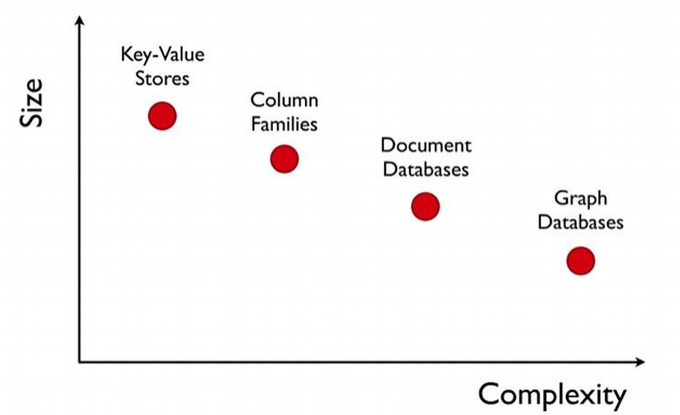
\includegraphics[scale=0.5]{IMAGE1.jpg}
\end{center}



\section{MongoDB}
MongoDB is as already mentioned a document based management system, with the data stored in Bson (Binary Json), and the access to data is possible thanks to indexes. Compared to the SQL DBs Mongo doesn't have the join feature. The name changes are:

\begin{center}
	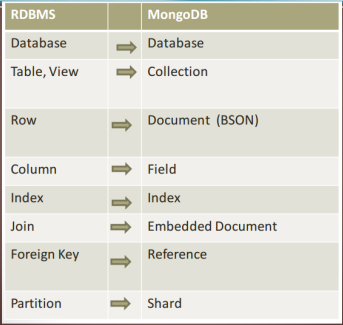
\includegraphics[scale=0.6]{IMAGE2.jpg}
\end{center}
In case of a massive data upload one might decide to:

\begin{itemize}[noitemsep]
	 
	\item
	Disable the acknowledgment(ack) of the data, which is a signal passed between communicating processes, computers or devices, to signify acknowledgment or receipt of message, as part of a communications
	protocol.
	\item
	Disable the writing on a log file
\end{itemize}

One must be attentive when doing so because any loss will not be registered and lost forever.

For large data-sets it is useful to use some additional structures called indexes, they are similar to the book indexes and act as a faster way to retrieve information, the might require more time during the insertion but makes the queries faster later, one primary index (basic one) is always the defined for the id. How does it exactly works?
Basically without an index Mongo will perform a simple table scan (like SQL) in which it has to look through all the ``book'' to find a query result, it is the same we would do if we didn't have the index for our books we will have to read it whole until finding the point where we
wanted to be. Indexing avoid this problem (more problematic if the database is large), it is an ordered list that points it's content.
Since indexing slows down the modifications one must choose just a couple of indexes for any given collection, the tricky part is to decide which one. Fact : MongoDB gives a limit of 64 indexes!

The aggregation uses pipeline and options. 
The aggregation pipeline starts processing the documents of the collection and passes the result to the next pipeline in order to get result for example: \$match and \$group. 
We can use the same operator in different pipelines.

Mongo for many reasons (mainly commercial) offers also a SQL interface, we need the connector BI (Business Intelligence) it generates the relational schema and use such schema to access the data.

\section{GraphDB}

What is a graph? It is a collection of nodes and edges which represents their relations. 
It has a lot of applications such as: social media, recommendations, Geo, Logistics network, financial transaction graphs (for fraud detection), master data management, Bioinformatics, authorization and access control.

The labeled property graph model has the following characteristics:

\begin{itemize}[noitemsep]
	 
	\item
	It contains nodes and relationships;
	\item
	Nodes contains properties (key : value pairs);
	\item
	Nodes can be labeled with one or many labels;
	\item
	Relationships are named and directed, with a start and end node;
	\item
	Relationships can contain properties like nodes.
	\item
	%magari migliorare questa parte
	The relationship can be fine-grained or generic: for example in case of Address we can choose distinct relationship like HOME\_ADDRESS or WORK\_ADDRESS or DELIVERY\_ADDRESS which is the fine-grained relationship or we could choose only address and specify in it which kind of address it is ADDRESS\{type : `home'\} or the other ones, this method is called generic relationship. Usually it's preferred the generic one especially in cases where I need to find all the address of a client all I need to do is find the ADDRESS relationship, in the fine-grained I needed to find one by one all kind of addresses, just	imagine if we had 100 types of addresses. On the other hand to find the DELIVERY\_ADDRESS all I need to do is find ADDRESS\{type:`delivery'\} 
\end{itemize}

A graph database (GD) can use either the native or non-native storage and processing engine.

Native Graph Storage is the one optimized for the native graph management \& the non native graph storage stores the data in non graph based model but this model supports a graph query language, examples: Relational, Object oriented DB, Wide Column, in a relational for example in a join bomb we can use a graph to connect two tables. But the problem
with the relational DBs and most of NoSQL DBs is that it lacks relationships.
Moreover in SQL joining tables adds more complexity, and in case of sparse table with null-able column require special checking in the code, in the case of a market, just to see what a customer bought we need to do a lot of expensive joins or the customers that buy a specific product with other products for the recommendation systems. 
For the NoSQL DBs whether key-value, document or column-oriented, we might use the aggregation technique to see the relationship, but the relationship between aggregates aren't citizen in the data model and is
costly operation since it's doesn't use index free adjacency, since they stay inside of aggregates with structure in form of nested maps and even after the aggregation there is no back link to point backward and run
other interesting queries.

In a native graph storage the attributes and nodes and the referenced nodes are stored together, to optimize the graph processing engine. 
When we perform a query the graph model does not depend on the total number of nodes instead it remain nearly constant because it works locally to the portion of the graph which is connected to the base node, while the other SQL and NoSQL models will suffer in performance speed with the
increase of data. Moreover we can add more data/nodes and relationship without disturbing the already existing model.

The processing engine uses index-free adjacency, meaning that connected nodes physically points to each other in the DB, this makes sure that the retrieval is faster but it comes at a cost, the efficiency of queries that do not use graph traversal, for example the writing time etc.

It's important to note that it's neither good nor bad to use native or non-native engine, simply one needs to choose one based on his/her needs, for example my DB is based on a non-graph backend (like MySQL) so it would be useful to use a non native graph storage.

The properties of the cypher language is :

\begin{enumerate}[noitemsep]
	 
	\item
	Pattern-matching Query language
	\item
	Humane language, easy to learn, read and understand
	\item
	Expressive yet compact
	\item
	Declarative : Say what you want, not how
	\item
	Borrows from well known query languages especially SQL, yet clearly it's different enough to see that it deals with graphs and not SQL	DBs.
	\item
	Aggregation, Ordering, Limit
	\item
	Update the Graph
\end{enumerate}

A real example is the following: We want to manage a server farm, we define a relational model for managing it. 
We know that a user access to application which runs on a VM and each application uses a DB and a secondary DB. 
Each of the VM is hosted on a server which are placed in a rack structure which is managed by a load balancer.

The initial stage of modeling is similar in any kind of DB, we seek to understand and agree on the entities in the domain and how to interrelate, usually done on whiteboard with a diagram which is a graph.
Next stage we seek a E-R (Entity-Relationship) diagram, which is another graph. 
After having a suitable logical model we map it into tables and relations. 
We keep are data in a relational DB, with it's rigid schema.
But keeping the data normalized slows down the query time so we need to denormalize it, because the user's data model must suit the database engine not the user. 
Denormalizing we involve duplicate data to gain query performance, denormalizing is not a trivial task and we accept that there may be substantial data redundancy. 
The problems doesn't stop here, because once created if we need to modify it, which we will need to do in order to match the changes in the production environment, so we will need to do this work all again!

It's better in there cases to directly use the graph DBs, it will avoid the data redundancy and it can adapt really fast in case of a change in the DB.

Another graph traversal language is Gremlin, part of the Apache TinkerPop framework. In this domain specific language (DSL) expressions specify a concatenation of traversal steps, so you basically explain to gremlin step by step what to do.

\section{Key-Value Model}

It's the most simple and flexible model of the NoSQL family, where every key is assigned to a value, it is possible to assign a type to a value.
The values are not query-able, such as a BLOB, where a BLOB(Binary Large OBject) is a collection of binary data stored as a single entity in a DB, for example images, videos etc.:
\begin{center}
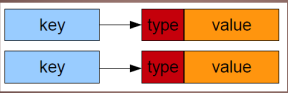
\includegraphics[scale=0.5]{IMAGE3.jpg}
\end{center}
An example is the amazon's cart system which uses DynamoDB a key-value system.

The basic operation in a key-valued models are:

\begin{itemize}[noitemsep]
	\item
	Insert a new key-value pair
	\item
	Delete a new key-value pair
	\item
	Update a new key-value pair
	\item
	Find a value given the key
\end{itemize}

There is no schema and the values of the data is opaque. The values can be accessed only through the key, and stored values can be anything : numbers, string, JSON, XML, images, binaries etc.
An example of key-value model is Riak and has the following terminology:
%Quanto è figo minipage, l'ho scoperto dopo aver cercato come unire una tabella con un immagine xD!
\begin{center}
	\begin{minipage}[b]{0.4\textwidth}
	\begin{tabular}{|l|l|}
		\hline
		\textbf{Relational} & \textbf{Riak}\\ \hline
		database instance & Riak cluster\\ \hline
		table & bucket \\ \hline
		row & key-value\\ \hline
		rowid & key\\ \hline
	\end{tabular}
	\end{minipage}
	\begin{minipage}{.5\textwidth}\centering
	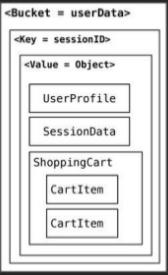
\includegraphics[scale=0.6]{IMAGE4.jpg}
	\end{minipage}

\end{center}
%Things not to remeber putting just for completation
Some other examples are: Redis, Memcached, Riak, Hazelcast, Encache.

Thanks to the Hash based index, the key-value systems can scale out in a very efficient way. 
The Hash is a mathematical function that assign to a given key it's value, usually we have h(x) = value, usually it returns a pointer to where the data is stored not exactly the data itself, for example h(x) = (x modulo y) where y is the max length of hash table. 
There might a problem with the conflicts but they can be managed. 
Hashing also enables items in the DB to be retrieved quickly. 
The hash table can be easily distributed in a network, it is managed in pile so we can have a key(saved in the pile) x saved in a server and it's succ(x) stored in a different server, thus scaling out really fast. 
The key value terminology is the following:

In a DHT(Distributed Hash Table) it is pretty simple to insert a key-value (k1,v1) basically take the key as input and route messages to the node holding that key and store the value there, and to retrieve the value of k1 it simply finds the node with the key k1 and return it's value v1 from it.

\section{Wide Column and BigTable}
This two models are an evolution, in a certain way, of the key-value models, when we start giving a structure to the value it becomes more complicated so we use wide column(Big Table): The first model was introduced by Google(HBase) and later on by Facebook (Cassandra) some think that Cassandra is still a key-value model and not a wide column.

BigTable is a multidimensional map, which can be accessed by row key, column key and a timestamp. It is sorted, persistent and sparse.
We will consider the \textbf{HBase BigTable} Model.
The data is organized in tables, each table(the tables are multi-versioned) is composed by the column-families that include columns, the cells within a column family are sorted physically and are usually very sparse with most of the cell having NULL value so we can have different rows with different sets of columns. 
BigTable is characterized by the row key, column key, timestamp, the row has the keys, column contains the data and contents. 
The column is divided in families. The timestamp support the multi-version of modification to check how the data changed over time and still be able to access the latest one without any confusion. We can represent it as follows:

\begin{center}
	\begin{tabular}{|c|c|c|}
		\hline
		\textbf{row key} & \textbf{column family 1} & \textbf{column family 2} \\
		\hline
		&
		\begin{tabular}{c|c}
			\textbf{column 1} & \textbf{column 2}
		\end{tabular}
		&
		\begin{tabular}{p{1.8cm}|p{1.8cm}|p{1.8cm}}
			\textbf{column 1} & \textbf{column 2} & \textbf{column 3}
		\end{tabular}
		\\
		\hline
		&
		\begin{tabular}{c|c}
		\textit{cell(data)} & \textit{cell(data)}
		\end{tabular}
		& 
		\begin{tabular}{p{1.8cm}|p{1.8cm}|p{1.8cm}}
		\textit{cell(data)}&\textit{cell(data)} &\textit{cell(data)}
		\end{tabular}\\
		\hline
		&
		\begin{tabular}{c|c}
			\textit{cell(data)} & \textit{cell(data)}
		\end{tabular}
		& 
		\begin{tabular}{p{1.8cm}|p{1.8cm}|p{1.8cm}}
			\textit{cell(data)}&\textit{cell(data)} &\textit{cell(data)}
		\end{tabular}\\
		\hline
	\end{tabular}\\
	~\\
	Each row can have different timestamp, so we can have more versions of this table.
\end{center}

The cells within The data is without type since it is saved in bytes. The columns are dynamic. So to get a data given a key we need to transform our data in Bytes with a comand .toBytes(``Key''), we can also use python to modify the columns via APIs. This model can be useful for *-To-Many mappings.
The row key is an array of bytes and serves as a primary key for the table.
Each Column Family has a name and contains one or more related columns, the columns can belong to one column family only and is included inside the row with familyName:columnName followed the value, for example we have: \\ 
%cavolo che sbatti i quote i LaTeX, se trovate un modo carino ditemelo
row key $|$ info:\{`height':`170cm', `state':`NY'\}  roles:\{`ASF':`Director', `Hadoop':`Founder'\}$|$\\
The version number of each row is unique within the row key, by default it uses the system's timestamp but they can be user supplied.

Best time to use HBase is when one need to scale out, need random write and/or read, when we need to do thousand of operations per second on multiple TB of Data, when we need to know all the modification done on
the data, when we need a well known and simple access. One can combine a GraphDB with HBase, one example is JanusGraph.
HBase does not support joins, but this can be done in application layer using Scan() and Get() operations of HBase.

\textbf{Cassandra}: It started as a support for the Facebook inbox search, it was open sourced in 2008 by Facebook and then it became a top-level project under Apache in 2010. The data model is the same as HBase, the only difference is the way it is stored (storage model) and the program algorithms. We can say it is a restricted BigTable, we can have only one column family. It uses a C* language very similar to SQL language.

Cassandra is a column oriented NoSQL system. 
The KeySpace is the outermost container, it's basic attributes are the Replication Factor (how many copies of the data we need), Replication Strategy and the Column Families.
The Column Families, can be seen as a collection of rows or better a collection of key-value pairs as rows. 
A row is a collection of columns labeled with a name, the value of a row is itself a sequence of key-value pairs where the keys are the column's name and we need at least one column in a row. The columns have the key(name), the value and the timestamp.
The Key Space is only a logical grouping of columns families.

\begin{center}
	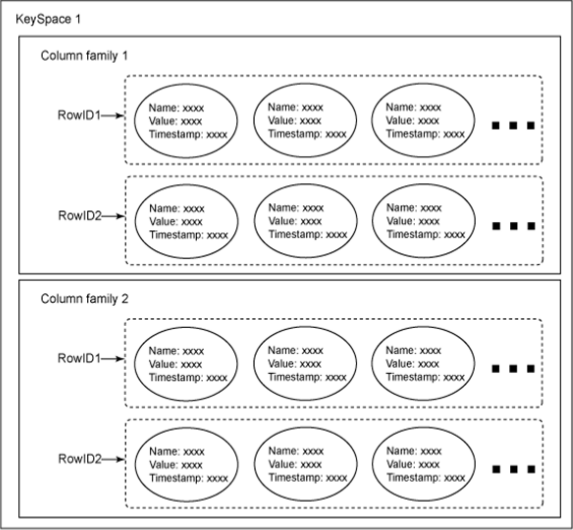
\includegraphics[scale=0.5]{IMAGE5.png}\\
	An example of Cassandra data model.
\end{center}

While with RDBMS, we can have that JOIN of normalized tables can return almost anything, with C* the data model is designed for specific queries and the schema is adjusted as new queries are introduced. In C* there are no JOINS, relationship or foreign keys and the data required by multiple tables are denormalized across those tables.

The Comparision between Apache Cassandra, Google Big Table and Amazon DynamoDB is:
\begin{center}
	\begin{tabular}{|p{3.6cm}|p{3.6cm}|p{3.3cm}|p{4cm}|}
		\hline
		&\textbf{Apache Cassandra} & \textbf{Google Big Table} & \textbf{Amazon DynamoDB}\\
		\hline
		\textit{Storage Type} & Column & Column & Key-Value\\
		\hline
		\textit{Best Use} & Write often\newline read less & Designed for\newline large scalability & Large database solution\\
		\hline
		\textit{Concurrency Control} & MVCC & Locks & ACID\\
		\hline
		\textit{Characteristics} & High Availability\newline Partition\newline Tolerance\newline Persistence & Consistency \newline High Availability\newline Partition\newline Tolerance \newline Persistence & Consistency \newline High Availability\\
		\hline
	\end{tabular}
\end{center}

%THIS ONE IS STILL A GIBBERISH I WILL IMPOROVE IT.
\section{Data Distribution}
If we divide our database into n databases, called the fragmentation of data, the bottom-lake phenomena arises in which the slowest machine becomes the bottom-lake and the max time for a query is dependent on that machine. 
Another way is to replicate the data 2 on 2 such as if a machine is not accessible we can have that data from another machine. We can also combine the fragmentation and replication.
The advantages of replication are:
\begin{itemize}[noitemsep]
	\item
	availability
	\item
	parallelism
	\item
	reduced data transfer.
\end{itemize}

while the disadvantages are:

\begin{itemize}[noitemsep]
	 
	\item
	increased cost of updates
	\item
	increased complexity of concurrency control e.g. two people book a ticket at the same time solution : {[}\ldots{}.{]}.
\end{itemize}

Data Transparency is very important so the users are not aware on the way we distribute the data.

Shared Everything : existed until 2000 (aprrox) we have one big complex costly data base shares everything and can be very slow, Share Disk : We have data saved on different disk connected between them,
no one uses it.

Share Nothing : every thing is separated it is very easy to scale out it Model used by noSQL models.

What to choose btwn Scaliblty or Avlblty? It depends on how much one wants to spend more availability means more money.

How to create replicas?
\begin{itemize}[noitemsep]
	\item take the data form master either the backup copy or the data itself	(if we can stop the activity of the server) and move it.
	\item Using log file : to maintain the replica as same as as the source even during the transfer (near real time).
\end{itemize}



%If you use Volume in project be attentive to the %scalability!!!!!

How MongoDB manages the distribution :

It uses Sharding : Every document has a key in mongodb so we define a shard key which defines the range of data. 
Example: Key is surname so we can decide all the surname staring from A to K save in first partition and
the other in the second.

The shard is basically a server so we need to use mongos (s=server) to make a querry on a shard.

What is a Shard exactly?

It's a node of the cluster, it can be a single monogod or a replica set. 
Mongodb also autometically replicates the data and in one shard I will have a primry chunk where I store the data I wanted and secondary chunks where mongo replicated other data as backup just in case, the secondary is a read only data so I cannot do update queries on it.

How to configure a mongoserver?

Mongod --configsvr

We can have different mongos on same pc on different ports.

What happens to the query?

For the target querry mongo selects the shard containing the data and then it's simplest

For the Scatter gather query we run query on all shard the collect the data and ``join'' it.

For the sorting we locally sort on all shards and the do a global sorting.

HBase each tool has a different terminology.

Hbase components is a subset of table's row (horizonal range partiton), which is automatcally done.

Hbase lives bcoz of ZooKeeper.

Hbase is similar to mongodb and have the same flaw : If the master is broken the client cannot obtain any data and we have an error.

Cassandra on the other hand repairs this flaw since there is no master and all the nodes are considered the same peer to peer.

In cassandra since I can add or remove nodes with no downtime we have a transparent elasticity and scalability and since it's P2P architecture we obtain also the High Availavility. 
Also cassandra uses ZooKeeper to find the replicas in other databases, given a node we decide the N number of following nodes in which the replica will we saved.

The data writing is separated in 3 stages : the first one is the log file writing which is essential, even if the data writing fails it doesn't matter bcoz we have the log file. 
And the consistency is based
on majority : if a certain number,which we decide, of the nodes agree that a certain data was written or read it is assumed to be true. 
Or use quorum which states the 50\% +1 nodes agree that something is written it's assumed true.

To delete the data is it easier to consider the data not available(like how recycle bin in OS), and follow it by compactation which reclaims the not available space.
\end{document}
